\documentclass[12pt]{article}
%\usepackage[vmargin=1.5cm, hmargin=1.5cm]{geometry}                
%\geometry{letterpaper}           
\usepackage[letterpaper, margin=1.87cm]{geometry}
%\usepackage{times}
\usepackage{graphicx, hanging, mdwlist, titlesec}
\usepackage{amssymb, fancyhdr, enumitem}
\usepackage{threeparttable, subfigure, multirow}
\usepackage{hyperref}
\usepackage{tikz}

%Header
\renewcommand{\headrulewidth}{0pt} 
\fancyhf{}
\lhead{\textbf{Matthew M Osmond} \textit{Curriculum Vitae}}
\rhead{\thepage}

\setitemize{noitemsep, topsep=1pt} %space bw items and bw paras and items in itemize enviro
\titlespacing{\subsection}{0pt}{*1}{*0}

\newcommand*{\ClipSep}{0.4cm}%

\begin{document}
\thispagestyle{empty} 
\pagestyle{fancy}

%%%%%%%%%%%%%%%%%%%%%%%%%%%%%%%%%%%%%%%%%%%%%%%%%%%%%%%%%%
%\begin{center}
{\raggedleft
\noindent\Large{\textbf{MATTHEW M.\ OSMOND}}\\
\large Postdoctoral Fellow\\
\large Center for Population Biology\\
\large University of California - Davis \\
\large mmosmond@ucdavis.edu\\
\href{https://mmosmond.github.io}{mmosmond.github.io}\\
%\end{center}
}

%\begin{tikzpicture}[remember picture,overlay]
%%sharp corners
%%\node[anchor = north west, yshift = -0.5cm, xshift=1.5cm] at (current page.north west) {\includegraphics[width=5cm]{ArnaudPlant}};
%%rounded corners
%\begin{scope}[xshift=-10, yshift = -10]
%    \clip [rounded corners=.5cm] (0,0) rectangle coordinate (centerpoint) ++(5cm,5cm); 
%    \node [inner sep=0pt] at (centerpoint) {\includegraphics[width=5.0cm]{IMAGES/ArnaudPlant}};
%\end{scope}
%\end{tikzpicture}

%%%%%%%%%%%%%%%%%%%%%%%%%%%%%%%%%%%%%%%%%%%%%%%%%%%%%%%%%%

%%%%%%%%%%%%%%%%%%%%%%%%%%%%%%%%%%%%%%%%%%%%%%%%%%%%%%%%%%%
%\section*{Research Interests}
%%%%%%%%%%%%%%%%%%%%%%%%%%%%%%%%%%%%%%%%%%%%%%%%%%%%%%%%%%%%
%
%I enjoy investigating how ecological and genetic factors influence the evolutionary process, and \textit{vice versa}.
%Recent/ongoing projects use mathematical models to investigate (\textit{i}) the role of sex and epistasis in shaping the genetic basis of evolutionary rescue, (\textit{ii}) the impact of haploid selection on the lability of sex determination systems, (\textit{iii}) the effect of species interactions on evolution and persistence in changing environments, and (\textit{iv}) how non-Mendelian inheritance affects the likelihood of crossing valleys of fitness created by epistasis.
%I am now building methods to infer eco-evolutionary dynamics from genomic data.
%Past projects involved actual fieldwork on real plant communities and wild birds.

%My past research was more empirical: I have helped explore how migration influences hybridization and speciation in the Swainson's thrush and Yellow-rumped warblers, the natural history of the endangered Kittlitz's murrelet in Alaska, plant community succession following wildfire in the boreal forests of Newfoundland, and the evolution of female colouration in a wild population of American redstarts.

%%%%%%%%%%%%%%%%%%%%%%%%%%%%%%%%%%%%%%%%%%%%%%%%%%%%%%%%%%
\section*{}
%%%%%%%%%%%%%%%%%%%%%%%%%%%%%%%%%%%%%%%%%%%%%%%%%%%%%%%%%%

\begin{tabular}{lll}
\textbf{Prof.} & Department of Ecology \& Evolutionary Biology, University of Toronto\hspace{0.5cm} & 2021-\\
\\
\textbf{PDF} & Center for Population Biology \& Banting Fellow, UC Davis & 2018-2020\\
& Mentors: Graham Coop, Sebastian Schreiber, Andrew Whitehead\\
\\
%\end{tabular}

%%%%%%%%%%%%%%%%%%%%%%%%%%%%%%%%%%%%%%%%%%%%%%%%%%%%%%%%%%
%\section*{Education}
%%%%%%%%%%%%%%%%%%%%%%%%%%%%%%%%%%%%%%%%%%%%%%%%%%%%%%%%%%

%\begin{tabular}{lll}
\textbf{PhD} & Zoology, University of British Columbia & 2013 - 2018\\
& Title: \textit{Adaptive challenges: fitness valleys and evolutionary rescue}\\
& Supervisor: Sarah Otto\\
& Committee: Amy Angert, Michael Doebeli, Michael Whitlock\\
\\
\textbf{MSc} & Biology, McGill University & 2010 - 2012 \\
& Title: \textit{Eco-evolutionary rescue: an adaptive dynamic analysis}  \\
& Supervisor: Claire de Mazancourt\\
& Committee: Michel Loreau, Fr\'{e}d\'{e}ric Guichard\\
\\
\textbf{BSc} &  Mathematics \& Biology, Queen's University & 2004 - 2008\\ %(83\% Avg.)
& Honours title: \textit{The meaning of female coloration in the American redstart}  \\
& Supervisors: Laurene Ratcliffe, Matt Reudink\\
& Committee: Paul Martin\\
\end{tabular}

%%%%%%%%%%%%%%%%%%%%%%%%%%%%%%%%%%%%%%%%%%%%%%%%%%%%%%%%%%
\section*{Selected Awards}
%%%%%%%%%%%%%%%%%%%%%%%%%%%%%%%%%%%%%%%%%%%%%%%%%%%%%%%%%%

\begin{tabular}{llr}
%  2020 & Young Investigator (Travel) Award, Society for Molecular Biology and Evolution & \\
  2019-2020 & Banting Postdoctoral Fellowship, Canada & \$140,000 \\
  2018-2020 & Center for Population Biology Postdoctoral Fellowship, UC Davis & \$125,000 \\
  2018-2020 & Postdoctoral Fellowship, NSERC (awarded but declined) & \$90,000 \\
%  2018 & Talk award, Evo-WIBO & a book\\ 
%  2017-2018 & Graduate Student Fellowship, University of British Columbia & \$16,500 \\
%  2017 & Zoology Graduate Student Travel Award, University of British Columbia \\%& \$500\\ 
%  2015 & Zoology Graduate Student Travel Award, University of British Columbia \\%& \$500\\ 
%  2015 & $2^{nd}$ best talk, Canadian Society for Ecology and Evolution Meeting & \$300\\ 
%  2013 & BRITE Travel Award, University of British Columbia \& NSERC \\%& \$500\\
%  2013 & International Research Mobility Award, University of British Columbia \\%& \$1,500\\ 
  2013-2017 & Alexander Graham Bell Canada Graduate Scholarship, NSERC & \$105,000\\
%  2013-2014 & Faculty of Science Graduate Award, University of British Columbia & \$6,000\\
%  2013-2018 & Four Year Fellowship, University of British Columbia & \$18,000\\
%  2013-2014 & BRITE Fellowship, University of British Columbia \& NSERC & \$6,000\\
  2011-2012 & Alexander Graham Bell Canada Graduate Scholarship, NSERC & \$17,500\\
  2011-2012 & Dr.\ Neal Simon Memorial Scholarship & \$1,000\\
%  2011-2012 & Excellence Award, Quebec Centre for Biodiversity Science & \$2,500\\
%  2011 & Graduate Research Enhancement and Travel Award, McGill University \\%& \$500\\
%  2010 & Provost's Graduate Fellowship, McGill University \\%& \$1,500\\
%  2010-2011 & Science and Technology Award, Ontario Graduate Scholarship & \$5,000\\
%  2009 & Faculty Research Scholarship, Lakehead University \\%& \$4,666\\
%  2008 & B.Sc.\ Honours with Distinction, Queen's University \\%& \$0 \\
%  2008 & Undergraduate Student Research Award (USRA), NSERC (declined) & \$4,500\\
  2007 & Undergraduate Student Research Award, NSERC & \$4,500\\
%  2005 & Annie Bentley Lillie Prize, First Year Calculus, Queen's University \\%& \$0\\
  %2004 - 2008 & Dean's Honour List, Queen's University\\
\end{tabular}

%\newpage
%%%%%%%%%%%%%%%%%%%%%%%%%%%%%%%%%%%%%%%%%%%%%%%%%%%%%%%%%%
\section*{Publications}
%%%%%%%%%%%%%%%%%%%%%%%%%%%%%%%%%%%%%%%%%%%%%%%%%%%%%%%%%%

\hangpara{1cm}{1}\noindent\hspace{.1cm}\textcolor{gray}{15. Lyberger K, \textbf{Osmond M}, Schreiber S. 2020. Is evolution in response to extreme events good for population persistence? \textit{bioR$\chi$iv} 10.1101/2020.04.02.014951.}

\hangpara{1cm}{1}\noindent\hspace{.1cm}14. Klausmeier C, \textbf{Osmond M}, Kremer C, Litchman E. 2020. Ecological limits to evolutionary rescue. \textit{Philosophical Transactions of the Royal Society B}. 375:20190453

\hangpara{1cm}{1}\noindent\hspace{.1cm}13. Henriques GJB, \textbf{Osmond M}. 2020. During environmental change, cooperation can promote rescue or lead to evolutionary suicide. \textit{Evolution} 74:1255-1273.

\hangpara{1cm}{1}\noindent\hspace{.1cm}12. \textbf{Osmond M}, Coop G. 2020. Genetic signatures of evolutionary rescue by a selective sweep. \textit{Genetics} 215:813-829.

\hangpara{1cm}{1}\noindent\hspace{.1cm}11. \textbf{Osmond M}, Otto SP, Martin G. 2020. Genetic paths to evolutionary rescue and the distribution of fitness effects along them. \textit{Genetics} 214:493-510.

\hangpara{1cm}{1}\noindent\hspace{.1cm}10. Thompson K, \textbf{Osmond M}, Schluter D. 2019. Parallel genetic evolution and speciation from standing variation. \textit{Evolution Letters} 3:129-141.

\hangpara{1cm}{1}\noindent\hspace{.1cm}9. Edwards K, Kremer C, Miller E, \textbf{Osmond M}, Litchman E, Klausmeier C. 2018. Evolutionary stable communities: a framework for understanding the role of trait evolution in the maintenance of diversity. \textit{Ecology Letters} 21:1853-1868.

\hangpara{1cm}{1}\noindent\hspace{.1cm}8. Scott M$^*$, \textbf{Osmond M}$^*$, Otto S. 2018. Haploid selection, sex ratio bias, and transitions between sex-determining systems. \textit{PLoS Biology} 16:e2005609. [$^*$ joint first authors]

\hangpara{1cm}{1}\noindent\hspace{.1cm}7. \textbf{Osmond M}, Klausmeier C. 2017. An evolutionary tipping point in a changing environment. \textit{Evolution} 71:2930-2941.

\hangpara{1cm}{1}\noindent\hspace{.1cm}6. \textbf{Osmond M}, Otto S, Klausmeier C. 2017. When predators help prey adapt and persist in a changing environment. \textit{The American Naturalist} 190:83-98. [F1000Prime Recommended]

\hangpara{1cm}{1}\noindent\hspace{.1cm}5. \textbf{Osmond M}, Barbour M, Bernhardt J, Pennell M, Sunday J, O'Connor M. 2017. Warming induced changes to body size stabilize consumer-resource dynamics. \textit{The American Naturalist} 189:718-725.

\hangpara{1cm}{1}\noindent\hspace{.1cm}4. Toews D, Delmore K, \textbf{Osmond M}, Taylor P, Irwin D. 2017. Migratory orientation in a narrow avian hybrid zone. \textit{PeerJ} 5:e3201.

\hangpara{1cm}{1}\noindent\hspace{.1cm}3. \textbf{Osmond M}, Otto S. 2015. Fitness-valley crossing with generalized parent-offspring transmission. \textit{Theoretical Population Biology} 105:1-16. %dx.doi.org/10.1016/j.tpb.2015.08.002.

\hangpara{1cm}{1}\noindent\hspace{.1cm}2. \textbf{Osmond M}, Reudink M, Marra P, Germain R, Nocera J,  Boag P, Ratcliffe L.  2013. Relationships between carotenoid-based female plumage and age, reproduction, and mate colour in the American Redstart. \textit{Canadian Journal of Zoology} 91:589-595. %dx.doi.org/10.1139/cjz-2013-0017.

\hangpara{1cm}{1}\noindent\hspace{.1cm}1. \textbf{Osmond M}, de Mazancourt C. 2013. How competition affects evolutionary rescue. \textit{Philosophical Transactions of the Royal Society B: Biological Sciences} 368:20120085. %dx.doi.org/10.1098/rstb.2012.0085.

%\vspace{0.25cm}
%\noindent\textit{Not peer reviewed}
%
%\hangpara{1cm}{1}\noindent\hspace{.1cm}Cragg J, Burger A, \textbf{Osmond M}. 2011.  Radar monitoring of \textit{Brachyramphus} murrelets on Kodiak Island, 2010. \textit{Report to the U.S. Geological Survey, Anchorage, Alaska}.

%\vspace{1cm}
%\subsubsection*{Preprints}

%\newpage
%%%%%%%%%%%%%%%%%%%%%%%%%%%%%%%%%%%%%%%%%%%%%%%%%%%%%%%%%%%
%\section*{Additional Research Experience}
%%%%%%%%%%%%%%%%%%%%%%%%%%%%%%%%%%%%%%%%%%%%%%%%%%%%%%%%%%%
%
%\begin{tabular}{ll}
%2017 & \textbf{Student} Evolutionary Quantitative Genetics workshop (J.\ Felsenstein \textit{et al.})\\
%2016 & \textbf{Visiting researcher} University of Montpellier and CNRS (O.\ Ronce, T.\ Lenormand)\\ 
%%2016 & \textbf{Participant} Stochastic Models in Evolution workshop (M.\ Kirkpatrick, T.\ Day, \textit{et al.}) \\
%2015 & \textbf{Student} Complex Systems Summer School (Santa Fe Institute)\\
%2013 &  \textbf{Student} Metacommunities summer school  (M.\ Leibold, C.\ Klausmeier)\\
%2013 &  \textbf{Researcher} Michigan State University (C.\ Klausmeier, E.\ Litchman)\\
%2012-2014 &  \textbf{Visiting researcher} University of Helsinki (S.\ Geritz, E.\ Kisdi)\\ 
%2012 &  \textbf{Research assistant} University of British Columbia (D.\ Irwin)\\
%2011 &  \textbf{Student} Adaptive Dynamics summer school  (S.\ Geritz, C.\ Klausmeier)\\
%2010-2012 &  \textbf{Member} Eco-evolutionary working group (A.\ Gonzalez \textit{et al.})\\
%2010 & \textbf{Research assistant} USGS (J.\ Piatt) and University of Victoria (A.\ Burger) \\
%2009-2010 & \textbf{MSc} (withdrew) Lakehead University (A.\ Mallik) \\
%%2007-2008 & \textbf{B.Sc.\ thesis} Queen's University (M.\ Reudink, L.\ Ratcliffe)
%\end{tabular}

%%%%%%%%%%%%%%%%%%%%%%%%%%%%%%%%%%%%%%%%%%%%%%%%%%%%%%%%%%
\section*{Service}
%%%%%%%%%%%%%%%%%%%%%%%%%%%%%%%%%%%%%%%%%%%%%%%%%%%%%%%%%%

\noindent \textbf{Reviewer} \textit{The American Naturalist} (11), \textit{Ecology Letters} (2), \textit{Evolution} (2), \textit{Genetics} (2), \textit{Journal of Theoretical Biology} (2), \textit{Theoretical Population Biology} (2), \textit{Biological Journal of the Lineann Society} (1), \textit{Ecology} (1), \textit{Ecology and Evolution} (1), \textit{eLife} (1), \textit{Frontiers in Ecology and Evolution} (1), \textit{Global Change Biology} (1), \textit{Heredity} (1), \textit{Molecular Biology and Evolution} (1), \textit{Nature Communications} (1), \textit{Nature Ecology and Evolution} (1), \textit{Philosophical Transactions of the Royal Society B} (1), \textit{Journal of Statistical Mechanics} (1), \textit{PLoS Computational Biology} (0.5), \textit{Science} (0.5)
%\begin{tabular}{ll}
%2018- & \textbf{Organizer} Center for Population Biology Seminar \& Social Hour, UC Davis \\
%2017-2018 & \textbf{Secretary} Zoology Graduate Student Society, University of British Columbia \\
%2017 & \textbf{Volunteer} Eco-Evo Retreat, Squamish, British Columbia \\
%2016-2017 & \textbf{Organizer} Let's Assume (evol.\ theory discussion group), University of British Columbia \\
%2014 & \textbf{Organizer} Vancouver Evolution Group (regional journal club), Vancouver \\
%2010-2012 & \textbf{Organizer} Eco-Theoretic Cafe (mathematical ecology discussion group), McGill University \\
%2007 & \textbf{Volunteer} Society of Canadian Ornithologists meeting,  Queen's University
%\end{tabular}

%%%%%%%%%%%%%%%%%%%%%%%%%%%%%%%%%%%%%%%%%%%%%%%%%%%%%%%%%%
%\section*{Teaching Experience/Training}
%%%%%%%%%%%%%%%%%%%%%%%%%%%%%%%%%%%%%%%%%%%%%%%%%%%%%%%%%%%
%
%\begin{tabular}{ll}
%2019 & \textbf{Participant} Teaching Toolkit for Diverse Learners, San Francisco State University\\ 
%2014, 2016, 2017 & \textbf{Marker} Population Genetics, University of British Columbia \\
%2011 & \textbf{Mentor} for work-study undergraduate student, McGill University \\
%2010 & \textbf{Teaching Assistant} Math Models in Biology, McGill University \\
%2010 & \textbf{Teaching Assistant} Organismal Biology, McGill University\\
%2010 &  \textbf{Teaching Assistant} Evolutionary Concepts, Lakehead University\\
%2009 &  \textbf{Teaching Assistant} Ecology, Lakehead University
%\end{tabular}

%%%%%%%%%%%%%%%%%%%%%%%%%%%%%%%%%%%%%%%%%%%%%%%%%%%%%%%%%%%
%\section*{Professional Membership}
%%%%%%%%%%%%%%%%%%%%%%%%%%%%%%%%%%%%%%%%%%%%%%%%%%%%%%%%%%%
%
%\noindent Genetics Society of America, 2018- \\
%\noindent American Society of Naturalists, 2014- \\
%\noindent Canadian Society for Ecology and Evolution, 2011-2013, 2015-

\newpage 
%%%%%%%%%%%%%%%%%%%%%%%%%%%%%%%%%%%%%%%%%%%%%%%%%%%%%%%%%%
\section*{Invited Seminars}
%%%%%%%%%%%%%%%%%%%%%%%%%%%%%%%%%%%%%%%%%%%%%%%%%%%%%%%%%%
\hangpara{0.5cm}{1}Osmond M. 2020. Evolutionary rescue: genetic basis and genetic signatures. Rescue Team online seminar series, \textbf{Max Planck Institute for Evolutionary Biology}, Pl\"{o}n, Germany. (virtual)

\hangpara{0.5cm}{1}Osmond M. 2018. Evolutionary rescue: adaptation, genetics, demography. \textbf{University of Toronto}, Toronto, Canada.

\hangpara{0.5cm}{1}Osmond M, Martin G, Ronce O, Otto S. 2018. Evolutionary rescue. Mathematical Biology Seminar, \textbf{University of British Columbia}, Vancouver, Canada.

\hangpara{0.5cm}{1}Osmond M. 2018. Evolutionary rescue: integrating ecological and evolutionary theory. Center for Population Biology, \textbf{University of California - Davis}, Davis, USA. 

\hangpara{0.5cm}{1}Osmond M, Martin G, Otto S, Ronce O. 2016. Genetic signatures of evolutionary rescue with sex. Stochastic Models for the Inference of Life Evolution group, \textbf{College de France}, Paris, France. 

\hangpara{0.5cm}{1}Osmond M, Otto S, Klausmeier C. 2016. When predators help prey adapt and persist. \textbf{Institute National de la Recherche Agronomique}, Montpellier, France. 

\hangpara{0.5cm}{1}Osmond M, Otto S. 2016. Subcritical adaptation: fitness valleys and evolutionary rescue. Stochastic and Deterministic Models for Evolutionary Biology workshop, \textbf{Oaxaca}, Mexico. 

%\hangpara{0.5cm}{1}\textbf{Osmond, M.}* and Otto, S.P., 2014. Crossing fitness-valleys without the help of Mendel. Talk, Biomathematics Group, University of Helsinki.

\hangpara{0.5cm}{1}Osmond M, de Mazancourt C. 2013. Using adaptive dynamics to predict evolution and extinction in changing environments. Pacific Institute for the Mathematical Sciences, \textbf{University of British Columbia}, Vancouver, Canada.

%\hangpara{0.5cm}{1}\textbf{Osmond M}*, de Mazancourt C. 2012. Using adaptive dynamics to predict evolution and extinction in changing environments. Talk, Biomathematics Group, University of Helsinki, Finland.

\hangpara{0.5cm}{1}Osmond M, de Mazancourt C. 2011. To adapt and persist in a changing environment. Mick Follows lab, \textbf{Massachusetts Institute of Technology}, Boston, USA.

%\newpage
%%%%%%%%%%%%%%%%%%%%%%%%%%%%%%%%%%%%%%%%%%%%%%%%%%%%%%%%%%
%\section*{Conference Presentations}
%%%%%%%%%%%%%%%%%%%%%%%%%%%%%%%%%%%%%%%%%%%%%%%%%%%%%%%%%%%
%
%\hangpara{0.5cm}{1}\textbf{Osmond M}, Coop G. 2020. Inferring the locations of genetic ancestors. American Naturalist, Asilomar, USA. (poster)
%
%\hangpara{0.5cm}{1}\textbf{Osmond M}, Coop G. 2019. Genetic signatures of evolutionary rescue. Evolution, Providence, USA.
%
%\hangpara{0.5cm}{1}\textbf{Osmond M}, Coop G. 2019. Genetic signatures of evolutionary rescue. Bay Area Population Genetics, Stanford, USA.
%
%\hangpara{0.5cm}{1}\textbf{Osmond M}, Martin G, Ronce O, Otto S. 2018. Genetic paths to evolutionary rescue. Population and Evolutionary Quantitative Genetics, Madison, USA. (poster) \textbf{*Poster award}
%
%%\hangpara{0.5cm}{1}\textbf{Osmond M}. 2018. Evolutionary rescue: integrating ecological and evolutionary theory. Talk, BLISS, UBC, Canada. 
%
%\hangpara{0.5cm}{1}\textbf{Osmond M}, Martin G, Ronce O, Otto S. 2018. Predicting the genetic paths evolutionary rescue will take. Evo-WIBO, Port Townsend, USA. \textbf{*Talk award}
%
%%\hangpara{0.5cm}{1}\textbf{Osmond M}. 2018. Predicting the genetic paths evolutionary rescue will take. Talk, Zoology Graduate Student Association Symposium, UBC, Canada.
%
%\hangpara{0.5cm}{1}\textbf{Osmond M}, Scott M, Otto S. 2017. Gametic competition, meiotic drive, sex ratio selection, and transitions between sex determination systems. Evolution, Portland, USA. 
%
%\hangpara{0.5cm}{1}\textbf{Osmond M}, Klausmeier C. 2017. Evolutionary tipping points in changing environments. Canadian Society for Ecology and Evolution, Victoria, Canada. 
%
%%\hangpara{0.5cm}{1}\textbf{Osmond M}*, Otto SP, and Klausmeier C. 2016. When predators help prey adapt and persist. Talk, Zoology Graduate Student Association Symposium, UBC, Canada. 
%
%\hangpara{0.5cm}{1}\textbf{Osmond M}, Otto S, Klausmeier C. 2016. When predators help prey adapt and persist. Evolution, Austin, USA. 
%
%\hangpara{0.5cm}{1}\textbf{Osmond M}, Klausmeier C. 2016. When predators help prey adapt and persist. Evo-WIBO, Port Townsend, USA.
%
%\hangpara{0.5cm}{1}\textbf{Osmond M}, Otto S. 2015. Crossing fitness-valleys without the help of Mendel: extending theory. Canadian Society for Ecology and Evolution, Saskatoon, Canada. \textbf{*Talk award}
%
%%\hangpara{0.5cm}{1}\textbf{Osmond, M.M.}* and Otto, S.P., 2014. Adapt or die. Poster, Eco-Evo Retreat, Squamish, BC.
%
%\hangpara{0.5cm}{1}\textbf{Osmond M}, Otto S. 2014. Crossing fitness-valleys without the help of Mendel. Evolution, Raleigh, USA. (poster)
%
%\hangpara{0.5cm}{1}\textbf{Osmond M}, Otto S. 2014. Crossing fitness-valleys without the help of Mendel. Evo-WIBO, Port Townsend, USA. (poster)
%
%%\hangpara{0.5cm}{1}\textbf{Osmond, M.}* and Otto, S.P., 2014. Crossing fitness-valleys without the help of Mendel. Poster, Zoology Graduate Student Association Symposium, UBC.
%
%\hangpara{0.5cm}{1}\textbf{Osmond M}, Otto S. 2014. Crossing fitness-valleys without the help of Mendel. Evolution of Mating Systems, University of Jyv\"askyl\"a, Jyv\"askyl\"a, Finland. (poster)
%
%%\hangpara{0.5cm}{1}\textbf{Osmond M}*, Klausmeier C, Litchman E. 2013. Predator-prey coevolution in a changing environment. Talk, Eco-Evo Retreat, Squamish, Canada.
%
%\hangpara{0.5cm}{1}\textbf{Osmond M}, Weigang H. 2012. Shorter generation times, slower evolution? Impact of life-history on evolution. Swedish Meeting on Mathematics in Biology, Lund, Sweden. (poster)
%
%\hangpara{0.5cm}{1}\textbf{Osmond M}, Weigang H. 2012. How life-history affects the rate of evolution. Biomathematics Day, University of Helsinki, Helsinki, Finland.
%
%\hangpara{0.5cm}{1}\textbf{Osmond M}, de Mazancourt C. 2012. How competition affects evolutionary rescue. Joint Congress on Evolutionary Biology, Ottawa, Canada.
%
%\hangpara{0.5cm}{1}\textbf{Osmond M}, de Mazancourt C. 2011. Evolutionary rescue and competition. Quebec Centre for Biodiversity Science Symposium, Montreal, Canada.
%
%\hangpara{0.5cm}{1}\textbf{Osmond M}, de Mazancourt C. 2011. To adapt and persist in a changing environment. Canadian Society for Ecology and Evolution, Banff, Canada. (poster)

%\hangpara{0.5cm}{1}\textbf{Osmond, M.}* and de Mazancourt, C., 2011. To adapt and persist in a changing environment. Talk, McGill Conservation, Ecology, Evolution, and Behaviour Symposium.

%\hangpara{0.5cm}{1}Rieder, R.*, Wheeler, J.A., Sutton, E., Kravchenko, D., \textbf{Osmond, M.}, Jacobs, J.D., Hermanutz, L., and Mallik, A.U., 2010. Nutrient bioavailability for black spruce establishment as influenced by elevation and post-fire disturbance. Poster, American Society of Agronomy and Soil Science Society of America Conference.

%\hangpara{0.5cm}{1}\textbf{Osmond, M.*} and Mallik, A.U., 2010. Pattern and stability of black spruce forest following wildfire.  Poster, Lakehead University Graduate Student Conference.

%\hangpara{0.5cm}{1}\textbf{Osmond, M.*} and Ratcliffe, L.M., 2008. Female plumage as a potential signal in the American redstart (\textit{Setophaga ruticilla}).  Poster, Queen's University Biology Poster Day.  

%\hangpara{0.5cm}{1}\textbf{Osmond, M.*} and Murphy, T.*, 2007. Ornithology in the Opinicon Region. Poster, Queen's University Biology Station Open House.



%%%%%%%%%%%%%%%%%%%%%%%%%%%%%%%%%%%%%%%%%%%%%%%%%%%%%%%%%%
%\section*{Selected Courses Taken}
%%%%%%%%%%%%%%%%%%%%%%%%%%%%%%%%%%%%%%%%%%%%%%%%%%%%%%%%%%

%
%\subsection*{Biology}                                          
%\noindent Biology of Cells, Biology of Organisms, Diversity of Life (I \& II), Mendelian and Molecular Genetics, Evolutionary Genetics, Population and Evolutionary Ecology, Plant Physiology, Animal Behaviour, Molecular Biology, Bioremediation, Conservation Biology, Research in Biology$^1$, Plant Ecology$^1$, Linking Community and Ecosystem Ecology$^1$ (Loreau), Advanced Evolutionary Ecology$^1$ (Hendry), Population ecology$^1$ (Angert), Bioinformatics for Evolutionary Biology$^1$
%\subsection*{Mathematical Biology}
%\noindent Applied Math Modeling, Modeling Techniques in Biology, Statistics for Genomics, Biostatistics$^1$, Adaptive Dynamics$^1$ (Geritz), Metacommunities$^1$ (Leibold), Population Genetics$^1$ (Whitlock), Evolutionary Quantitative Genetics$^1$ (Felsenstein)
%\subsection*{Mathematics}
%\noindent Differential Equations, Linear Algebra (I \& III), Differential and Integral Calculus, Advanced Calculus, Rings and Fields, Probability, Stochastic Processes and Applications, Operations Research, Statistics
%\subsection*{Other}
%\noindent Fundamental Questions (philosophy), General Chemistry, Organic Chemistry (I \& II), Religion and Social Ethics, Modern Middle East, Philosophy and Postmodernism, Writing Science Articles$^1$, Complex Systems Summer School$^1$ (Sante Fe Institute)
%\footnotetext[1]{Graduate course}

%\begin{tabular}{lll}
%2017 & Evolutionary Quantitative Genetics & J.\ Felsenstein, S.\ Arnold, \textit{et al.}\\
%2016 & Bioinformatics for Evolutionary Biology & G.\ Owens, K.\ Hodgins\\
%2015 & Complex Systems Summer School & Sante Fe Institute\\
%2015 & Population Ecology & A.\ Angert\\
%2013 & Population Genetics & M.\ Whitlock\\
%2013 & Metacommunities & M.\ Leibold \& C.\ Klausmeier\\
%2012 & Advanced Evolutionary Ecology & A.\ Hendry\\
%2011 & Adaptive Dynamics & S.\ Geritz \& C.\ Klausmeier\\
%2010 & Linking Community and Ecosystem Ecology & M.\ Loreau\\
%\end{tabular}
%
%%%%%%%%%%%%%%%%%%%%%%%%%%%%%%%%%%%%%%%%%%%%%%%%%%%%%%%%%%
%\section*{Programming Languages}
%%%%%%%%%%%%%%%%%%%%%%%%%%%%%%%%%%%%%%%%%%%%%%%%%%%%%%%%%%
%\noindent \textit{Mathematica}, \LaTeX, \texttt{python}, \textsf{R}, UNIX 


%\newpage
%%%%%%%%%%%%%%%%%%%%%%%%%%%%%%%%%%%%%%%%%%%%%%%%%%%%%%%%%%
%\section*{Other Interests}
%%%%%%%%%%%%%%%%%%%%%%%%%%%%%%%%%%%%%%%%%%%%%%%%%%%%%%%%%%

%\begin{figure}[!h]
%\centering
%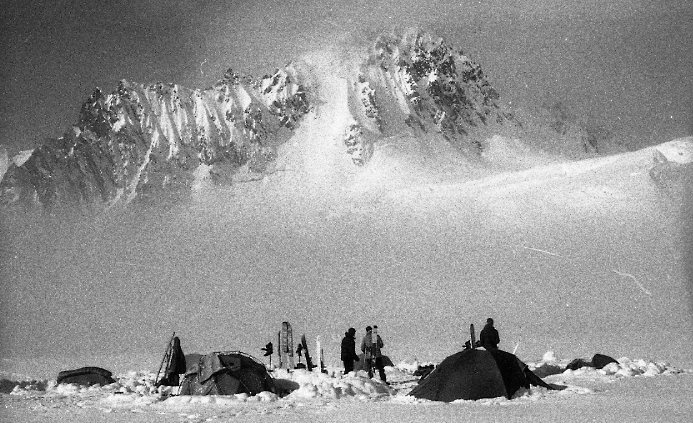
\includegraphics[width=0.45\linewidth]{IMAGES/Haines}
%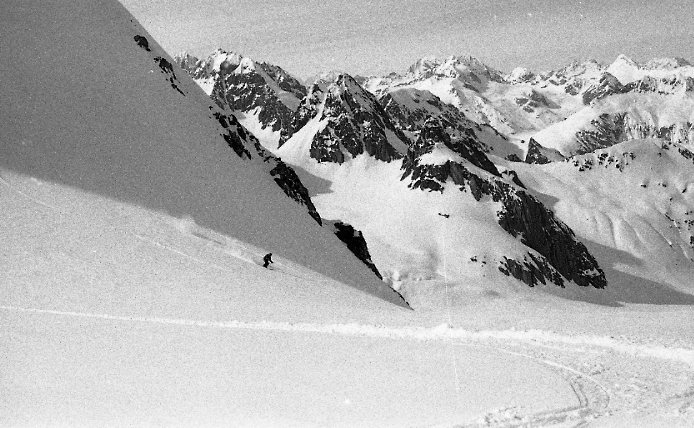
\includegraphics[width=0.45\linewidth]{IMAGES/SkiHaines}
%\vspace*{-1cm}
%\end{figure}

\end{document}